\chapter{运动学}
\label{ch:Kinematics in Straight Line}
运动学是整个物理学最早研究的现象。但是其实有的时候物体到底有没有动这都是并不明确的。比较著名的有悖论有飞矢不动悖论

\section*{学习目标}
\begin{todolist}
	\item 理解距离和速率的标量性质,位移、速度和加速度的矢量性质
	\item 绘制$d-t$图,$v-t$图以及从这些运动图像中求算其他物理量
	\item 利用\textbf{匀加速直线运动}的公式,解决问题
	\item 掌握位移,速度,加速度之间存在的求导和积分的关系,并利用微积分解决复杂运动学问题
\end{todolist}

\clearpage


\section{基础概念}
\label{sec:Basic Concepts}
因此从定量的角度进行研究的话,首先需要明确的是\gls{rframe}的概念。只有先指定\gls{rframe}之后才可以描述物体的运动状态。否则就是否定了运动的相对性


\subsection*{位置、距离和位移}
\label{subsec:Positiosn,Distantce,Displacement}
位置或者\gls{positionvec}是一个瞬时状态物理量。
但是\gls{distance}和\gls{displacement} 都是过程量,其中距离为标量,位移为矢量。一个物体的运动必须持续\textcolor{r1}{一段时间}才能够产生位移或者运动距离。

一个运动物体过程中的位置,距离和位移关系如下图所示:
\begin{figure}[H]
	\centering
	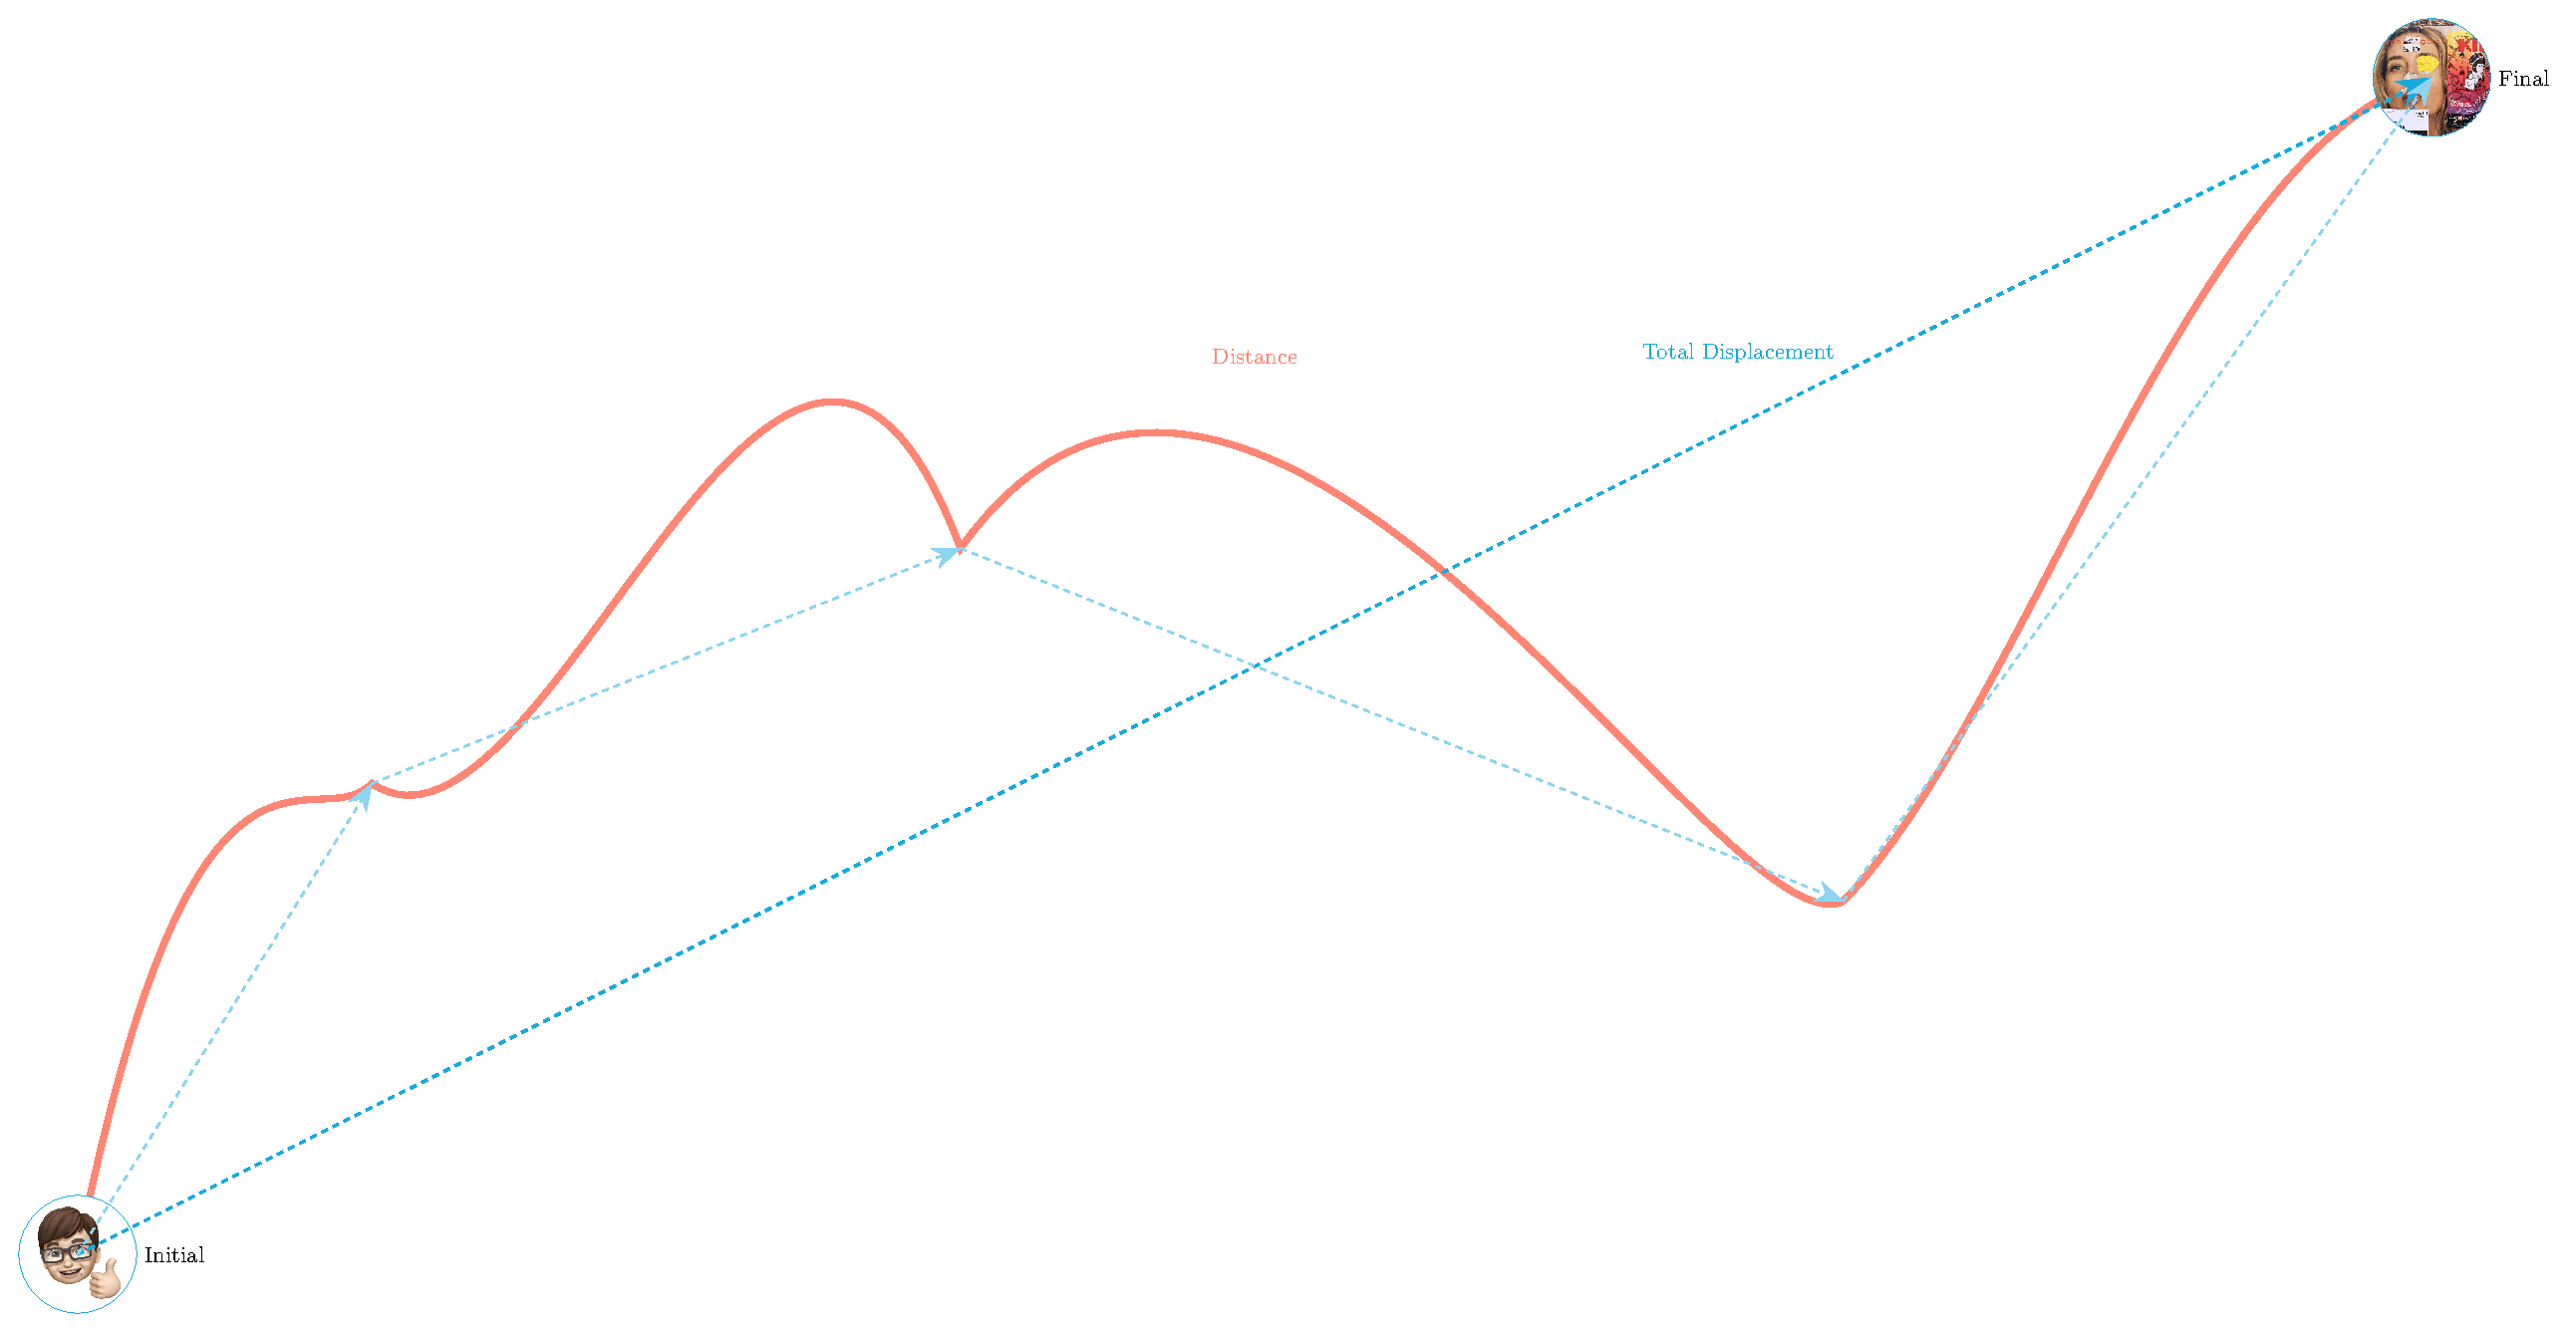
\includegraphics[width=0.8\textwidth]{movingpath}
	\caption{运动轨迹和分段位移}
\end{figure}
不过,我们肯定先从最简单的\gls{linearmotion}开始研究。


\subsection*{速度与速率}
\label{subsec:Velocity vs Speed}
\gls{speed}是标量,\gls{velocity}是矢量。这两者速度的定义通过\textcolor{r1}{位移除以时间}来求算,因此有\textcolor{r1}{一段时间的平均速度}的求算
\[
	v=\frac{\mathrm{d}elta x}{\mathrm{d}elta t}
\]
以及\textcolor{r1}{任意时刻的}\gls{insv}的求算
\[
	v=\frac{\mathrm{d} x(t)}{\mathrm{d} t}
\]
而瞬时速率仅仅是瞬时速度的大小而已,不需要陈述其方向。

先看一维方向的线性运动,比较简单。先规定\textcolor{r1}{正方向}。这样就可以用+/-表示方向了。如下图
\begin{figure}[H]
	\centering
	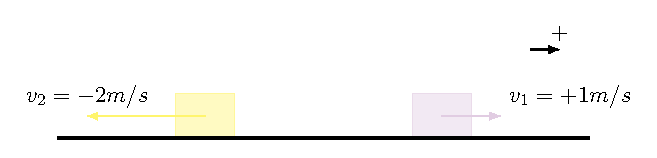
\includegraphics[width=0.8\textwidth]{direction}
	\caption{线性速度的矢量性可以通过正负号体现}
\end{figure}


\subsection*{加速度}
\label{subsec:Acceleration}
现在我们需要研究的物理量越来越少了,还剩下最后一个描述运动的物理量-\gls{acc}。在实际生活中,比如公交车启动的过程,任意时刻公交车的瞬时速度必然不可能保持一致,因此和推导速度的过程一致,定义出加速度的概念来研究速度变化的快慢。因此有点类似于一个套娃--\emph{速度的变化率}是加速度。
\[
	a= \frac{\mathrm{d}elta v}{\mathrm{d}elta t} =\frac{\mathrm{d} v}{\mathrm{d} t}
\]


\clearpage


\section{运动图像}
\label{sec:Graphs of motion}
之前有很重要的概念,就是位移,速度和加速度这是三个都是瞬时状态物理量,因此单纯用文字的方式很难描述一个运动过程的全部时刻的\emph{瞬时}位移,速度和加速度。但是,数学函数的表达式或者图像却可以做到这件事,因此,当我们把一段时间内\emph{每一个时刻}的位移,速度和加速度都采用坐标系的方式标注出来的话,我们就得到了非常经典的运动学图像了。

比如一个经典的静止的运动图像:

\begin{figure}[H] %pdfpages调用出问题。
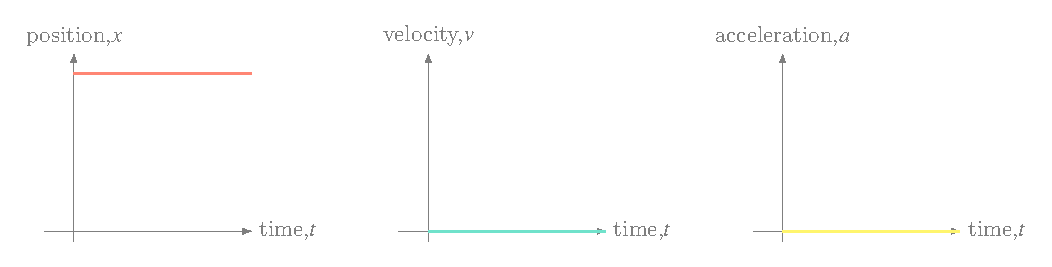
\includegraphics[page=1,width=0.8\textwidth]{dva-t.pdf}
\caption{静止不动的物体}
\end{figure}

再比如一个简单的匀速直线运动的图像:

\begin{figure}[H]  %这个图片包不太行
\includegraphics[page=2,width=0.8\textwidth]{dva-t.pdf}
\caption{做匀速直线运动的物体}
\end{figure}

但是,先暂停一下,$x-t$,$v-t$,和$a-t$之间有没有什么关联性呢?但是必定是有的,根据之前所述。$v=\frac{\mathrm{d}elta x}{\mathrm{d}elta t}$或者瞬时速度$v=\frac{\mathrm{d} x}{\mathrm{d} t}$因此,根据$x-t$的斜率,不就可以求算出瞬时速度的大小了吗?同理可得,$v-t$图像上的斜率就是加速度$a$的大小。因此匀速直线运动的图像就形成了如上图所示的特征。

最后再看一下匀加速直线运动的图像:
\begin{figure}[H]
\includegraphics[page=3,width=0.8\textwidth]{dva-t.pdf}
\label{fig:uniform acc}
\caption{做匀加速直线运动的物体}
\end{figure}

\begin{TaskBox}
在\ref{fig:uniform acc}的$x-t$图像中,寻找速度为$0$的时刻,并指出在$v-t$图像中对应的时刻。
\end{TaskBox}

\subsection*{运动学中的微积分}
正如之前所说,利用微分,可以根据位移信息推断速度;再次利用微分,可以从速度当中推算加速度;这是正向思路,逆向思路也是行得通的。因为积分和微分是互为逆运算的关系。因此得知加速度$a$可以通过积分求算速度的变化量$\mathrm{d}elta v$,当提供初速度之后,就可确定每一个时刻的速度也就是$v-t$关系;那么再通过一次积分就可以求算位移了。

因此,无论是再复杂的运动,只需要提供$s$,$v$,$a$当中任意一个随时间的函数关系,就可以推导其他的物理量。运动学当中的微分和积分的关系可以概括如下:
\begin{figure}[H]
\centering
\includegraphics[width=0.8\textwidth]{sva.png}
\caption{一路顺边不停积分,反向求导}
\end{figure}

\begin{ExampleBox}
A particle $P$ moves in a straight line passing through a point $O$. At time $t$\si{\s}, the acceleration, $a$\si{\m \per \square \s} , of $P$ is given by $a = 6 − 0.24t$. The particle comes to instantaneous rest at time $t = 20$.\\
(i) Find the value of $t$ at which the particle is again at instantaneous rest.\\
(ii) Find the distance the particle travels between the times of instantaneous rest\\
\makebox{}\hfill adapted from 2018 spring qp42 Q6

\tcblower
(i) 由于给定了加速度,因此可以求算v-t关系
\begin{align*}
	 v(t) &= \int a \mathrm{d} t \\
	  &=6t-0.12t^2+C
\end{align*}
将$v=0,t=20$带入可得 $v(t)=-0.12t^2+6t-72$
因此解方程$-0.12t^2+6t-72=0$得到$t=20$ or $t=30$\\

(ii)由于求算了$v(t)$关系,因此继续积分可以求算位移
\begin{align*}
	s &= \int_{20}^{30} v(t) \mathrm{d} t\\
	&= \int_{20}^{30} (-0.12t^2+6t-72) \mathrm{d} t\\
	&=-0.04t^3+3t^2-72t\bigg|^{20}_5\\
	&=20
\end{align*}
\end{ExampleBox}
\clearpage

\section{匀加速直线运动}
\label{sec:Constant Acceleration in a Straight Line}
那么现在再处理匀加速直线运动,这种加速度恒定的运动就非常简单了。首先我们回顾一下匀加速直线运动的$v-t$图:
\begin{figure}[H]
\centering
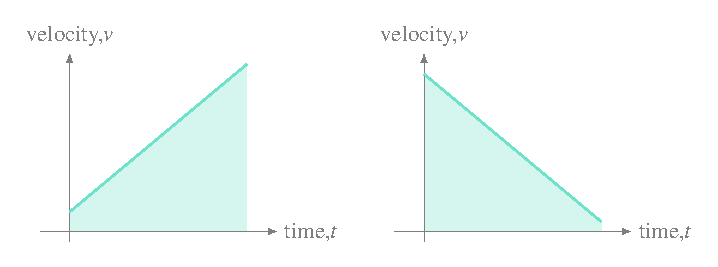
\includegraphics[width=0.8\textwidth]{unimotion}
\caption{匀加速度直线运动的图像}
\end{figure}

对于这样简单的$v-t$图,我们的分析还是沿用微积分的思想:
\begin{SummBox}
1. $v-t$图的斜率就是\textbf{加速度}\\
2. $v-t$图的包围面积就是\textbf{位移}
\end{SummBox}

因此,我们可以推导如下的公式:
\begin{table}[H]
\centering
\begin{tabular}{p{0.2\textwidth}p{0.2\textwidth}p{0.2\textwidth}}
$a=\frac{v-u}{t}$      & $t=\frac{v-u}{a}$      & $v=u+at$                 \\ 
$s=ut+\frac{1}{2}at^2$ & $s=vt-\frac{1}{2}at^2$   & $s=\frac{u+v}{2}\cdot t$ \\ 
$s=\frac{v^2-u^2}{2a}$ & $a=\frac{v^2-u^2}{2s}$ &                           
\end{tabular}
\end{table}

本质上这些公式只不过是把五个运动有关的物理量联系在一起的公式,这五个量分别是初速度$u$,末速度$v$,过程中恒定的加速度$a$,运动时间$t$,以及运动过程中的位移$s$。

在运用这些公式的时候,一定要注意$a$和$v$的方向性,与规定的方向相同使用+,相反则用-。比如对于自由落体情景,取$a=g=9.81$\si{\m\per\square \s},认定向下为正方向。

但是对于竖直上抛场景,则令$a=g=-9.81$ \si{\m\per\square \s}。认定竖直向上为正方向。这里方向的规定并不是强制的,但是一定要再利用这些公式进行求算之前就需要规定好。且严格按照规定方向确定速度以及加速度的正负号。
对于竖直上抛场景,到\textcolor{r1}{轨迹最高点}处的时候可以认为\textcolor{r1}{瞬时速度为0},通常是一个隐含条件。即使题目中不进行陈述,也是可以直接用的。

